\renewcommand\thesection{\Alph{section}}
\renewcommand\thesubsection{\thesection.\arabic{subsection}}
\setcounter{section}{5}
\section{Entrega final}

\setcounter{subsection}{1}
\subsection{Implementar el manejo de excepciones capturando errores potenciales específicos mediante Try-catch}

Lorem ipsum dolor sit amet, consectetur adipiscing elit. Donec et sem luctus, finibus mauris eget, euismod arcu. Morbi at mollis risus. Praesent consequat justo tellus, ac pretium urna lacinia quis. Ut sagittis cursus finibus. Morbi pellentesque vulputate tincidunt. Aliquam at pretium tellus, et vehicula velit. Nunc turpis metus, porttitor sit amet aliquam ut, venenatis quis elit. Nam tincidunt venenatis tortor, ac sodales libero varius nec. Donec vestibulum leo a metus rutrum, vitae elementum diam suscipit. Quisque non mauris rutrum, lacinia lectus id, viverra dui. In leo quam, ultrices vitae suscipit quis, porttitor quis turpis. Vestibulum semper ligula sit amet diam scelerisque gravida.

\subsection{Crear 2 clases que extiendan de una Excepción y que se utilicen en el programa}

Lorem ipsum dolor sit amet, consectetur adipiscing elit. Donec et sem luctus, finibus mauris eget, euismod arcu. Morbi at mollis risus. Praesent consequat justo tellus, ac pretium urna lacinia quis. Ut sagittis cursus finibus. Morbi pellentesque vulputate tincidunt. Aliquam at pretium tellus, et vehicula velit. Nunc turpis metus, porttitor sit amet aliquam ut, venenatis quis elit. Nam tincidunt venenatis tortor, ac sodales libero varius nec. Donec vestibulum leo a metus rutrum, vitae elementum diam suscipit. Quisque non mauris rutrum, lacinia lectus id, viverra dui. In leo quam, ultrices vitae suscipit quis, porttitor quis turpis. Vestibulum semper ligula sit amet diam scelerisque gravida.

\subsection{Aplicación del patrón de diseño Strategy (Estrategia)}

Lorem ipsum dolor sit amet, consectetur adipiscing elit. Donec et sem luctus, finibus mauris eget, euismod arcu. Morbi at mollis risus. Praesent consequat justo tellus, ac pretium urna lacinia quis. Ut sagittis cursus finibus. Morbi pellentesque vulputate tincidunt. Aliquam at pretium tellus, et vehicula velit. Nunc turpis metus, porttitor sit amet aliquam ut, venenatis quis elit. Nam tincidunt venenatis tortor, ac sodales libero varius nec. Donec vestibulum leo a metus rutrum, vitae elementum diam suscipit. Quisque non mauris rutrum, lacinia lectus id, viverra dui. In leo quam, ultrices vitae suscipit quis, porttitor quis turpis. Vestibulum semper ligula sit amet diam scelerisque gravida.

\subsubsection*{Opcional: Reemplazar los datos iniciales en el código por una conexión con base de datos local (MySQL), archivo de texto CSVo Excel, para la persistencia de datos}
\addcontentsline{toc}{subsubsection}{Opcional: Reemplazar los datos iniciales en el código por una conexión con base de datos local (MySQL), archivo de texto CSVo Excel, para la persistencia de datos}

Para la preservación de los datos poseemos tanto una carpeta en el proyecto (\textbf{Datafile}) con archivos csv, que nos permite el manejo de datos en formato local. Y también tenemos una conexión a una base de datos (\textbf{MySQL})

\begin{figure}[h]
    \centering
    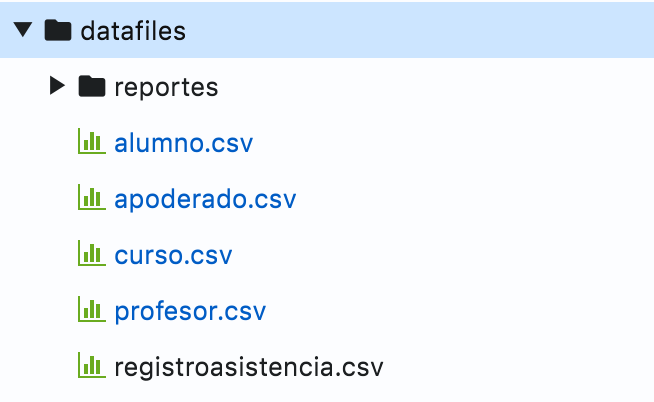
\includegraphics[width=0.35\textwidth]{contents/img/img12}
    \caption{Gestión de archivos CSV}
    \label{fig:img12}
\end{figure}

\clearpage

\begin{figure}[h]
    \centering
    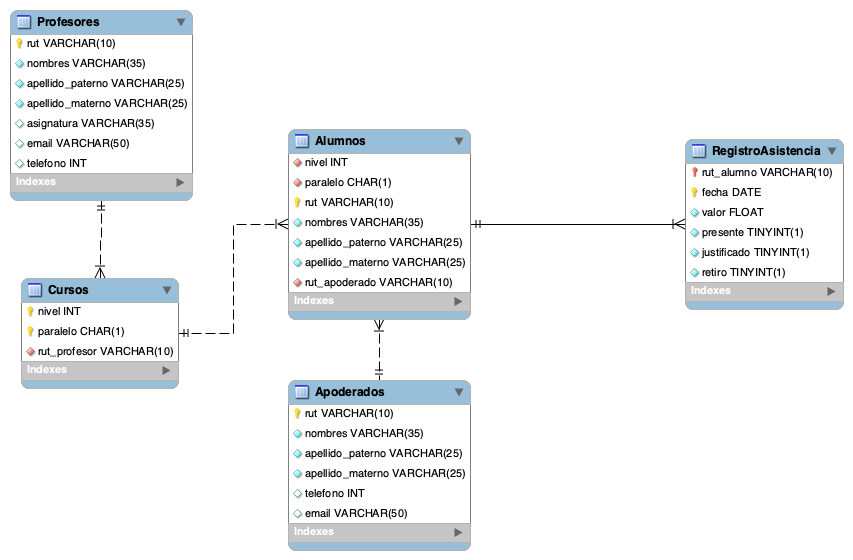
\includegraphics[width=1\textwidth]{contents/img/img13}
    \caption{Modelo de datos BD}
    \label{fig:img13}
\end{figure}

\subsubsection*{Opcional: Considerar la implementación del patrón Modelo-Vista-Controlador (MVC) en la arquitectura del sistema}
\addcontentsline{toc}{subsubsection}{Opcional: Considerar la implementación del patrón Modelo-Vista-Controlador (MVC) en la arquitectura del sistema}

Nuestro programa como se puede apreciar en la siguiente imagen  esta estructurado en un formato de modularización, en el cual separamos las clases y sus paquetes correspondientes  en un patrón MVC (Modelo-Vista-Controlador).

\begin{figure}[h]
    \centering
    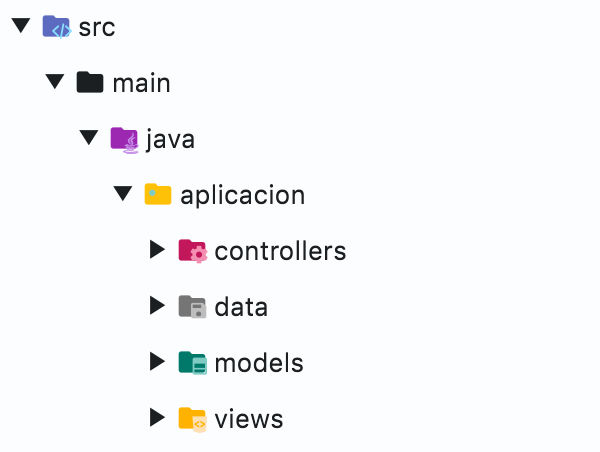
\includegraphics[width=0.35\textwidth]{contents/img/img14}
    \caption{Gestión de archivos para modelo MVC}
    \label{fig:img14}
\end{figure}
